\documentclass[sigconf,edbt,table]{acmart-edbt2021}

\def\BibTeX{{\rm B\kern-.05em{\sc i\kern-.025em b}\kern-.08em
    T\kern-.1667em\lower.7ex\hbox{E}\kern-.125emX}}

\usepackage{booktabs} % For formal tables
\usepackage{tikz}
\usepackage[noend]{algpseudocode}
\usepackage{algorithm}
\usepackage{algorithmicx}
\usepackage{xcolor}

\usepackage{multirow}

%\usepackage{colortbl}
\usepackage{subcaption}
\usepackage{listings}
\usepackage{extarrows}
\usetikzlibrary{shapes,shapes.geometric,fit,automata,positioning}
\usetikzlibrary{decorations.pathmorphing}
\tikzset{snake it/.style={decorate, decoration=snake}}

%\definecolor{lightgray}{gray}{0.9}

\newcommand{\cho}[1]{{\color{red} #1}}

% Copyright
\setcopyright{rightsretained}

% DOI
\acmDOI{}

% ISBN
\acmISBN{XXXXXXXX}

%Conference
\acmConference[EDBT 2021]{24th International Conference on Extending Database Technology (EDBT)}{March 23-26, 2021}{Nicosia, Cyprus}
\acmYear{2021}

\settopmatter{printacmref=false, printccs=false, printfolios=false}

\pagestyle{empty} % removes running headers

% Math square brackets
\DeclareMathOperator{\rank}{rank}
\makeatletter
\newenvironment{sqcases}{%
  \matrix@check\sqcases\env@sqcases
}{%
  \endarray\right.%
}
\def\env@sqcases{%
  \let\@ifnextchar\new@ifnextchar
  \left\lbrack
  \def\arraystretch{1.2}%
  \array{@{}l@{\quad}l@{}}%
}
\makeatother

% Footnote reference
\makeatletter
\newcommand\footnoteref[1]{\protected@xdef\@thefnmark{\ref{#1}}\@footnotemark}
\makeatother

\newcommand\gsv[2]{{\color{red}{#1}( {#2} $^{\text{gsv}}$)}}

\tikzset{elliptic state/.style={draw,ellipse}}

\begin{document}
\title{Multiple-Source Context-Free Path Querying in Terms of Linear Algebra}
% \begin{document}
% \title{Implementing support for context-free path queering for the Cypher extension in RedisGraph}
% \titlenote{Produces the permission block, and copyright information}
% \subtitle{Extended Abstract}
% \subtitlenote{The full version of the author's guide is available as
%   \texttt{acmart.pdf} document}



\author{Arseniy Terekhov}
	\email{simpletondl@yandex.ru}
	\affiliation{%
		\institution{Saint Petersburg State University}
		\streetaddress{7/9 Universitetskaya nab.}
		\city{St. Petersburg}
		\country{Russia}
		\postcode{199034}
	}

\author{Vlada Pogozhelskaya}
	\email{pogozhelskaya@gmail.com}
	\affiliation{%
		\institution{Saint Petersburg State University}
		\streetaddress{7/9 Universitetskaya nab.}
		\city{St. Petersburg}
		\country{Russia}
		\postcode{199034}
	}

\author{Vadim Abzalov}
	\email{vadim.i.abzalov@gmail.com}
	\affiliation{%
		\institution{Saint Petersburg State University}
		\streetaddress{7/9 Universitetskaya nab.}
		\city{St. Petersburg}
		\country{Russia}
		\postcode{199034}
	}

\author{Timur Zinnatulin}
	\email{!!!@!!!}
	\affiliation{%
		\institution{Saint Petersburg State University}
		\streetaddress{7/9 Universitetskaya nab.}
		\city{St. Petersburg}
		\country{Russia}
		\postcode{199034}
	}

\author{Semyon Grigorev}
	\email{s.v.grigoriev@spbu.ru}
	\email{semyon.grigorev@jetbrains.com}
	\orcid{0000-0002-7966-0698}
	\affiliation{
		\institution{Saint Petersburg State University}
		\streetaddress{7/9 Universitetskaya nab.}
		\city{St. Petersburg}
		\country{Russia}
		\postcode{199034}
	}
	\affiliation{
		\institution{JetBrains Research}
		\streetaddress{Primorskiy prospekt 68-70, Building 1}
		\city{St. Petersburg}
		\country{Russia}
		\postcode{199034}
	}

% The default list of authors is too long for headers}
% \renewcommand{\shortauthors}{B. Trovato et al.}
\renewcommand{\shortauthors}{Arseniy Terekhov et al.}


\begin{abstract}
Context-Free Path Querying (CFPQ) allows one to use context-free grammars to express paths constraints in navigational graph queries.
Algorithms for CFPQ studied actively for a long time, but no one graph database provide full-stack support of CFPQ.
In this work we provide multiple-source version of Azimov's CFPQ algorithm, which, as shown by Arseniy Terekhov is applicable for real-world graph analysis.
This step allows us to make the algorithm more practical and integrate it into RedisGraph graph database.
In order to provide full-stack support we also implement Cypher graph query language extension that allows one to express context-free constraints.
As a result, we provide the first, in our knowledge, full-stack support of CFPQ for graph database.
Our evaluation shows that the provided solution is applicable for real-world graph analysis.
\end{abstract}

%
% % The code below should be generated by the tool at
% % http://dl.acm.org/ccs.cfm
% % Please copy and paste the code instead of the example below.
% %
\begin{CCSXML}
		<ccs2012>
		<concept>
			<concept_id>10002951.10002952.10003197.10010825</concept_id>
			<concept_desc>Information systems~Query languages for non-relational engines</concept_desc>
			<concept_significance>500</concept_significance>
		</concept>
		<concept>
			<concept_id>10003752.10003766.10003771</concept_id>
			<concept_desc>Theory of computation~Grammars and context-free languages</concept_desc>
			<concept_significance>500</concept_significance>
		</concept>
		<concept>
			<concept_id>10002950.10003624.10003633.10003640</concept_id>
			<concept_desc>Mathematics of computing~Paths and connectivity problems</concept_desc>
			<concept_significance>300</concept_significance>
		</concept>
		<concept>
			<concept_id>10002951.10002952.10002953.10010146</concept_id>
			<concept_desc>Information systems~Graph-based database models</concept_desc>
			<concept_significance>500</concept_significance>
		</concept>
		</ccs2012>
\end{CCSXML}

    \ccsdesc[500]{Information systems~Graph-based database models}
	\ccsdesc[500]{Information systems~Query languages for non-relational engines}
	\ccsdesc[500]{Theory of computation~Grammars and context-free languages}
    \ccsdesc[300]{Mathematics of computing~Paths and connectivity problems}


% \keywords{ACM proceedings, \LaTeX, text tagging}

%% A "teaser" image appears between the author and affiliation
%% information and the body of the document, and typically spans the
%% page.
%\begin{teaserfigure}
%  \includegraphics[width=\textwidth]{new_hope.png}
%  \caption{Episode IV: A New Hope}
%  \label{fig:teaser}
%\end{teaserfigure}

\maketitle

\section{Introduction}

Scalable high-performance graph analysis is an actual challenge.
There is a big number of ways to attack this challenge~\cite{Coimbra2021} and the first promising idea is to utilize general-purpose graphic processing units (GPGPU).
Such existing solutions, as CuSha~\cite{10.1145/2600212.2600227} and Gunrock~\cite{7967137} show that utilization of GPUs can improve the performance of graph analysis, moreover it is shown that solutions may be scaled to multi-GPU systems.
But low flexibility and high complexity of API are problems of these solutions.

The second promising thing which provides a user-friendly API for high-performance graph analysis algorithms creation is a GraphBLAS API~\cite{7761646} which provides linear algebra based building blocks to create graph analysis algorithms.
The idea of GraphBLAS is based on a well-known fact that linear algebra operations can be efficiently implemented on parallel hardware.
Along with that, a graph can be natively represented using matrices: adjacency matrix, incidence matrix, etc.
While reference CPU-based implementation of GraphBLAS, SuiteSparse:GraphBLAS~\cite{10.1145/3322125}, demonstrates good performance in real-world tasks, GPU-based implementation is challenging.

One of the challenges in this way is that real data are often sparse, thus underlying matrices and vectors are also sparse, and, as a result, classical dense data structures and respective algorithms are inefficient. 
So, it is necessary to use advanced data structures and procedures to implement sparse linear algebra, but the efficient implementation of them on GPU is hard due to the irregularity of workload and data access patterns.
Though such well-known libraries as cuSPARSE show that sparse linear algebra operations can be efficiently implemented for GPGPU, it is not so trivial to implement GraphBLAS on GPGPU. 
First of all, it requires \textit{generic} sparse linear algebra, thus it is impossible just to reuse existing libraries which are almost all specified for operations over floats.
The second problem is specific optimizations, such as masking fusion, which can not be natively implemented on top of existing kernels.
Nevertheless, there is a number of implementations of GraphBLAS on GPGPU, such as GraphBLAST~\cite{yang2019graphblast}, GBTL~\cite{7529957}, which show that GPGPUs utilization can improve the performance of GraphBLAS-based graph analysis solutions.
But these solutions are not portable because they are based on Nvidia Cuda stack.
Moreover, the scalability problem is not solved: all these solutions support only single-GPU, not multi-GPU computations.

To provide portable GPU implementation of GraphBLAS API we developed a \textit{SPLA} library\footnote{Source code available at: \url{https://github.com/JetBrains-Research/spla}}.
This library utilizes OpenCL for GPGPU computing to be portable across devices of different vendors.
Moreover, it is initially designed to utilize multiple GPGPUs to be scalable.
To sum up, the contribution of this work is the following.
\begin{itemize}
    \item Design of portable GPU GraphBLAS implementation proposed. The design involves the utilization of multiple GPUS. Additionally, the proposed design is aimed to simplify library tuning and wrappers for different high-level platforms and languages creation. 
    \item Subset of GraphBLAS API, including such operations as masking, matrix-matrix multiplication, matrix-matrix e-wise addition, is implemented. The current implementation is limited by COO and CSR matrix representation format and uses basic algorithms for some operations, but work in progress and more data formats will be supported and advanced algorithms will be implemented in the future.
    \item Preliminary evaluation on such algorithms as breadth-first search (BFS) and triangles counting (TC), and real-world graphs shows portability across different vendors and promising performance: for some problems Spla is comparable with GraphBLAST. Surprisingly, for some problems, the proposed solution on embedded Intel graphic card shows better performance than SuiteSparse:GraphBLAS on the respective CPU. At the same time, the evaluation shows that further optimization is required.
\end{itemize} 
\section{Preliminaries}

In this section we introduce common definitions in graph theory and formal language theory which will be used in this paper. 
Also, we provide brief description of Azimov's algorithm which is used as a base of our solution.

\subsection{Graphs}

In this work we use edge-labelled digraph as a data model and define it as follows.
\begin{definition} \emph{Labeled directed graph} is a triple $D = (V,E,\sigma)$, where
\begin{itemize}
    \item $V$ is a set of vertices
    \item $E$ is a set of edges
    \item $\sigma \subseteq \Sigma$ is a set of labels, and a set of edges $E\subseteq V\times \sigma \times V$
\end{itemize}
\end{definition}

An example of the graph is presented in figure~\ref{fig:example_input_graph}.

\begin{figure}[h]
    \centering        
    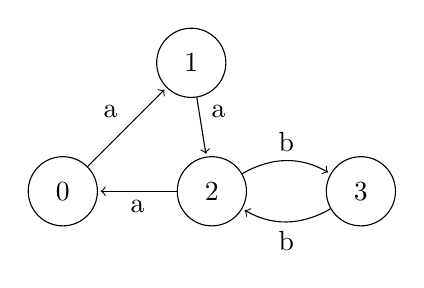
\begin{tikzpicture}[shorten >=1pt,auto]
       \node[state] (q_0)                      {$0$};
       \node[state] (q_1) [above right=of q_0] {$1$};
       \node[state] (q_2) [right=of q_0]       {$2$};
       \node[state] (q_3) [right=of q_2]       {$3$};
        \path[->]
        (q_0) edge  node {a} (q_1)
        (q_1) edge  node {a} (q_2)
        (q_2) edge  node {a} (q_0)
        (q_2) edge[bend left, above]  node {b} (q_3)
        (q_3) edge[bend left, below]  node {b} (q_2);
    \end{tikzpicture}
    \caption{The example of input graph $\mathcal{G}$}
    \label{fig:example_input_graph}
\end{figure}

We use adjacency matrix decomposed to a set of a boolean matrix as a representation of the graph.
\begin{definition}
An adjacency matrix $M$ of the graph $\mathcal{G}=$ is a square $|V|\times|V|$ matrix, such that $M[i,j] = \{l \mid e = (i,l,j) \in E\}$.
\end{definition}

Adjacency matrix $M$ of the graph $\mathcal{G}$ is

$$
    M =
    \begin{pmatrix}
    . & \{a\} & . & .     \\
    . & . & \{a\} & .     \\
    \{a\} & . & . & \{b\} \\
    . & . & \{b\} & .
    \end{pmatrix}.
$$

\begin{definition}

Boolean decomposition of adjacency matrix $M$ of graph $\mathcal{G}=$ is set of Boolean matrix $$\mathcal{M} = \{M^l \mid l \in L, M^l[i,j]=1 \iff l \in M[i,j]\}.$$

\end{definition}

Matrix $M$ can be represented as a set of two Boolean matrices $M^a$ and $M^b$ where
\begin{align}
M^{a} =
\begin{pmatrix}
    . & 1 & . & .   \\
    . & . & 1 & .   \\
    1 & . & . & .   \\
    . & . & . & .  
\end{pmatrix}, 
M^{b} =
\begin{pmatrix}      
    . & . & . & .   \\
    . & . & . & .   \\
    . & . & . & 1   \\
    . & . & 1 & . 
\end{pmatrix} \label{eq:boolean_decomposition_of_graph}
\end{align}
\subsection{Languages}

\begin{definition}\emph{Context-free grammar} is a 4-tuple $G=(N, \Sigma, R, S)$, where 
\begin{itemize}
    \item $N$ is a set of nonterminals
    \item $\Sigma$ is a set of terminals
    \item $R$ is a finite set of productions of the followings form: $A \to \alpha, ~A \in N,~ \alpha \in (N \cup \Sigma)^*$
    \item $S$ - a starting nonterminal
\end{itemize}
\end{definition}

\begin{definition} \emph{Context-free language} is a language generated by a context-free grammar:
\begin{align*}
     L(G) = \{w \in \Sigma^* \mid S \Rightarrow^* w \} 
\end{align*}
Where $S \Rightarrow^* w$  denotes that a string $w$ can be generated from a starting non-terminal $S$ using some sequence of production rules from $P$.
\end{definition}

\begin{definition} Context-free grammar $G = (N, \Sigma, R, S)$ is said to be in \emph{Chomsky normal form} if all productions in $R$ are of the form:
    \begin{itemize}
        \item $A \rightarrow BC,~A,~B,~C \in N$
        \item  $A \rightarrow a,~A \in N,~a \in \Sigma$
        \item $S \rightarrow \varepsilon,~\varepsilon$ is an empty string
    \end{itemize}
\end{definition}
Note that every context-free grammar can be transformed into an equivalent one in Chomsky Normal Form. 
\begin{definition} Context-free grammar $G = (N, \Sigma, P, S)$ is said to be in \emph{Weak Chomsky normal form} if all productions in $P$ are of the form:
    \begin{itemize}
        \item $A \rightarrow BC,~A,~B,~C \in N$
        \item  $A \rightarrow a,~A \in N,~a \in \Sigma$
        \item $A \rightarrow \varepsilon,~A \in N$
    \end{itemize}
\end{definition}
In other words, weak Chomsky normal form differs from Chomsky normal Form in the followings:
\begin{itemize}
    \item $\varepsilon$ can be derived from any non-terminal
    \item $S$ can be at a right part of productions
\end{itemize}
    
    
For example, let's consider the following context-free grammar, which generates the language $L(G) = \{A^nB^n, n \in \mathbb{N}\}$:
$G=(N, \Sigma, P, S), ~N=\{S\},~\Sigma=\{A,B\}$ and productions: 
\begin{align*}
S \rightarrow AB \\
S \rightarrow ASB\\
S \rightarrow \varepsilon
\end{align*}
After transformation to Chomsky Normal Form the resulting grammar:
\begin{align*}
S \rightarrow AB \\
S \rightarrow AC \\
C \rightarrow SB \\
S \rightarrow \varepsilon
\end{align*}

This productions itself are the grammar that has the same result as original grammar.

We use a context-free grammar in the weak Chomsky Normal Form without a starting non-terminal, which will be specified in the path queries for the graph. It should be noted that we omit the rules of the form $A \rightarrow \varepsilon$ for the reason that they correspond to trivial paths, which are more convenient to consider separately.

\begin{definition}\emph{Context-free relation} is a relation $R_A \subseteq V \times V$ for graph $G = (V, E)$, context-free grammar $G = (N,~\Sigma,~P)$ and fixed non-terminal $A$:
\begin{align*}
     R_A = \{(n, m) \mid \exists n \pi m~(l(\pi) \in L(G_A))\}
\end{align*}
\end{definition}

 Now, the definition for \emph{multiple-source (single-source) context-free path querying problem} can be formulated in the introduced notation as follows. For the given graph $G = (V, E)$, context-free grammar $G=(N, \Sigma, P)$ and set of source vertices $Src$ we need to find all context-free relations $R_A$ for any $A \in Src$. 
 
\subsection{Matrix-Based Algorithm}
Let $D = (V, E)$ be the input graph and $G = (N, \Sigma, P)$ be the input grammar. For the context-free path query evaluation, we need to provide context-free relations \mbox{$R_A \subseteq V \times V$} for every \mbox{$A \in N$}.
The matrix-based algorithm for CFPQ can be expressed in terms of operations over Boolean matrices (see listing~\ref{alg:algo0}) which is an advantage for implementation.
{\footnotesize
\begin{algorithm}
\begin{algorithmic}[1]
\caption{Context-free path querying algorithm}
\label{alg:algo0}
\Function{evalCFPQ}{$D=(V,E), G=(N,\Sigma,P)$}
    \State{$n \gets$ |V|}
    \State{$T \gets \{T^{A_i} \mid A_i \in N, T^{A_i}$ is a matrix $n \times n$, $T^{A_i}_{k,l} \gets$ \texttt{false}\} }
    \ForAll{$(i,x,j) \in E$, $A_k \mid A_k \to x \in P$}
        %\Comment{Matrices initialization}
        %\For{$A_k \mid A_k \to x \in P$}
          {$T^{A_k}_{i,j} \gets \texttt{true}$}
        %\EndFor
    \EndFor
    \ForAll{$A_k \mid A_k \to \varepsilon \in P$}
        \ForAll{$i \in \{0,\ldots ,n-1\}$}
            {$T^{A_k}_{i,i} \gets \texttt{true}$}
        \EndFor
    \EndFor

    \While{any matrix in $T$ is changing}
        %\Comment{Transitive c	losure calculation}
        \For{$A_i \to A_j A_k \in P$}
          { $T^{A_i} \gets T^{A_i} + (T^{A_j} \times T^{A_k})$ } 
        \EndFor
    \EndWhile
\State \Return $T$
\EndFunction
\end{algorithmic}
\end{algorithm}
}

This CFPQ algorithm allows efficiently apply GPGPU techniques, but it solves all-pairs problem and takes unreasonable amount of memory in scenarios in which we want to find paths from a relatively small set of vertices, since it calculates a lot of redundant information.  
\section{Matrix-based multiple-source CFPQ algorithm}

 In this section we introduce two versions of multiple-source matrix-based CFPQ algorithm. This algorithm is a modification of Azimov's matrix-based algorithm for CFPQ and the idea is that we cut off those vertices from which we are not interested in paths.
 
 Let \mbox{$D = (V, E)$} be the input graph, \mbox{$G = (N, \Sigma, P, S)$} be the input grammar and $Src$ be the input set of vertices. For the multiple-source context-free path query evaluation, we must provide such a path from $R_A$ where the start node is from $Src$. In other words, for every \mbox{$n \in Src$} we want to find all node pairs \mbox{$(n,m)$} such that \mbox{$\exists n \pi m~(l(\pi) \in L(G_A))$}.

\begin{algorithm}
\floatname{algorithm}{Listing}
\begin{algorithmic}[1]
\caption{Multiple-source context-free path querying algorithm}
\label{lst:algo1}
\Function{MultiSrcCFPQ}{$D=(V,E), G=(N,\Sigma,P,S), Src$}
    \State{$T \gets \{T^A \mid  A \in N, T^A \gets \emptyset\}$}
    \Comment{Matrix in which every element is $\emptyset$}
    
    \State{$TSrc \gets \{TSrc^A \mid  A \in N \setminus S, TSrc^A \gets \emptyset\}$}
    \Comment{Matrix for input vertices in which every element is $\emptyset$}

    \ForAll{$ v \in Src$} \Comment{Input matrix initialization}
        \State{$TSrc^S_{v,v} \gets true$} 
    \EndFor

    \ForAll{$A \to x \in P$} \Comment{Simple rules initialization}
        \ForAll{$(v, x, to) \in E$}
            \State{$T^A_{v,to} \gets true$}
        \EndFor
    \EndFor

    \While{$T\ or\ TSrc\ is\ changing$} \Comment{Algorithm's body}
        \ForAll{$A \to B C \in P$}
            \State{$M \gets TSrc^A*T^B$}
            \State{$T^A \gets T^A + M*T^C$}
            \State{$TSrc^B \gets TSrc^B + TSrc^A$}
            \State{$TSrc^C \gets TSrc^C + $ \Call{getDst}{M}}
        \EndFor
    \EndWhile
    \State \Return T
\EndFunction

\\

\Function{getDst}{M}
    \State{$A \gets \emptyset$}
    \ForAll{$(v,to) \in V^2 \mid M_{v,to} = true$}
        \State{$A_{to,to} \gets true$}
    \EndFor
    \State \Return A
\EndFunction
\end{algorithmic}
\end{algorithm}

The operation of transitive closure calculation from Azimov's algorithm is supplemented with one more matrix multiplication which saves only vertices we are interested in.

It is useful to add data caching to improve the performance of processing large graphs. We provide one more version of algorithm which has memory optimization. It is noticed that every time we want to find all paths from the certain set of vertices, the first version of algorithm calculates everything from scratch. Since recalculating might take the significant amount of time, the second version is specified for such scenarios. This version stores all the vertices, the paths from which have already been calculated. 
\begin{algorithm}
\floatname{algorithm}{Listing}
\begin{algorithmic}[1]
\caption{Optimized multiple-source context-free path querying algorithm}
\label{lst:algo1}
\Function{MultiSrcCFPQSmart}{$index=(D, G, T, TSrc), Src$}
    \State{$TNewSrc \gets \{TNewSrc^A \mid  A \in N \setminus S, TNewSrc^A \gets \emptyset\}$}

    \ForAll{$v \in Src \mid index.TSrc_{v,v} = false$}
        \State{$TNewSrc^S_{v,v} \gets true$}
    \EndFor

    \While{$index.T\ or\ TNewSrc\ is\ changing$}
        \ForAll{$A \to B C \in P$}
            \State{$M \gets TNewSrc^A*index.T^B$}
            \State{$index.T^A \gets index.T^A + M*index.T^C$}

            \State{$TNewSrc^B \gets TNewSrc^B + TNewSrc^A \setminus index.TSrc^B$}
            \State{$TNewSrc^C \gets TNewSrc^C + $ \Call{getDst}{M}} $\setminus$ $index.TSrc^C$
        \EndFor
    \EndWhile
\EndFunction


\end{algorithmic}
\end{algorithm}

\subsection{Implementation Details}
 All of the above versions have been implemented$\footnote{GitHub repository with implemented algorithms: \url{https://github.com/JetBrains-Research/CFPQ_PyAlgo}, last accessed 28.08.2020}$ using GraphBLAS framework that allows you to represent graphs as matrices and work with them in terms of linear algebra. For convenience, all the code is written in Python using pygraphblas\footnote{GitHub repository of PyGraphBLAS library: \url{https://github.com/michelp/pygraphblas}}, which is Python wrapper around GraphBLAS API and based on SuiteSparse:GraphBLAS\footnote{GitHub repository of SuiteSparse:GraphBLAS library: \url{https://github.com/DrTimothyAldenDavis/SuiteSparse}}~\cite{SuiteSparse} --- the full implementation of GraphBLAS standart. This library is specialized for working with sparse matrices, which most often appear in real graphs.

\subsection{Algorithm Evaluation}

And comparison. With combinators, GLL (.NET version).

Evaluation setup.
Hardware basic description.

Graphs and queries from CFPQ\_Data\footnote{!!!}
Graphs and queries description: \#V, \#E, types of queries.

Tables.

Graphics (boxes). 1,2,4,8,16,32,50,100,500,1000,5000

Results.

Conclusion. 
\section{CFPQ Full-Stack Support}

In order to provide full-stack support of CFPQ it is necessatry to choose an appropriate graph database.
It was shown by Arseniy Terekhov et al. in~\cite{10.1145/3398682.3399163} that matrix-based algorithm can be naturally integrated into RedisGraph graph database because both, the algorithm and the database, operates over matrix representation of graphs.
Moreover, RedisGraph supports Cypher as a query language and there is a proposal which describes Cypher extension which allows one to specify context-free constraints.
Thus we choose RedisGraph as a base for our solution.  


\subsection{Cypher Extending}
\label{subsec:cypher-extension}

The first what we should do is to extend Cypher parser to be able to express context-free constraints.
There is a description of the respective Cypher syntax extension\footnote{\label{cypher-proposal}Formal syntax specification: \url{https://github.com/thobe/openCypher/blob/rpq/cip/1.accepted/CIP2017-02-06-Path-Patterns.adoc\#11-syntax}. Access date: 19.07.2020.}, proposed by Tobias Lindaaker, but this syntax does not implement yet in Cypher parsers.

This extension introduces path patterns, which are powerful alternative to the original Cypher relationship patterns.
Path patterns allow one to express regular constrains over basic patterns such as relationship and node patterns.
Like relationship patterns, they can be specified in the \texttt{MATCH} clause.

Main feature which allows one to specify context-free constraints is a \textit{named path patterns}: one can specify a name for path pattern and after that use this name in other patterns, or in the same pattern.
Named patterns can be defined in the \texttt{PATH PATTERN} clause.
Using this feature, structure of query is pretty similar to context-free grammar in the Extended Backus-Naur Form (EBNF)~\cite{EBNF_ISO}.

\begin{algorithm}
\floatname{algorithm}{Listing}
\begin{algorithmic}[1]
\caption{Query based on example grammar $G_1$ (eq.~\ref{eqn:g1_example}) in Cypher with path patterns}
\label{lst:cypher_example}
\State PATH PATTERN S = ()-/ [:c $\sim$S :d] | [:c (:y) :d] /->()
\State MATCH (v:x)-[:a | :c]->()-/ :b $\sim$S /->(to)
\State RETURN v, to
\end{algorithmic}
\end{algorithm}


The example of query which uses named path patters is presented in listing~\ref{lst:cypher_example}. 
This query is based on context-free grammar $G_1$ (eq.~\ref{eqn:g1_example}). 
Namely, path patter with name \texttt{S} specifies exactly the same constraint that specified by the grammar $G_1$. 
The \texttt{MATCH} clause uses pattern \texttt{S} in complex constraint which says that path of interest should starts in the vertex with label \texttt{x}, than in should goes throw edge with label \texttt{a} or \texttt{c}, and the end of path is a sequence of edges which starts from \texttt{b} and tail of this sequence matches with \texttt{S}.  

For the example graph $D_1$ this query returns the next pairs of vertices \texttt{(v, to)} (as specified in \texttt{RETURN} clause): !!!!

Thus this Cypher extension allows one express more complex queries including context-free path queries.
RedisGraph database supports subset of Cypher language and uses \texttt{libcypher-parser}\footnote{The \texttt{libcypher-parser} is an open-source parser library for Cypher query language. GitHub repository of the project: \url{https://github.com/cleishm/libcypher-parser}. Access date: 19.07.2020.} library to parse queries.
We extend this library by introducing new syntax proposed.
Note that we implement\footnote{The modified libsypher-pareser library with support of syntax for path patterns: \url{https://github.com/YaccConstructor/libcypher-parser}. Access date: 19.07.2020.} full extension, not only part which is necessary for simple CFPQ. 

\subsection{RedisGraph Extending}

This section describes the implementation of support for executing queries with the extended syntax in the RedisGraph. Throughout this section, we consider executing the example query from listing~\autoref{lst:cypher-example-3} for the graph $D_1$ from~\autoref{fig:example_input_graph}. $\mathcal{E}$ and $\mathcal{V}$ denotes boolean decompositions of adjacency and vertex label matrices of $D_1$ respectively. 

In the RedisGraph the main part of processing a query is building its execution plan. Execution plan consists of operations that perform basic processing such as filtering, pattern matching, aggregation and result construction. The diagram of its construction is shown in~\autoref{fig:execution-plan-construction}. It can be divided into two parts ---\gsv{processing named and unnamed path patterns, which are described below}{Improve it!}.

 In the first stage of processing, these patterns turn into an intermediate representation --- the \textit{query graph}. The nodes and edges of the query graph corresponds to node and relationship patterns. We extended query graph to be able to contain path patterns. Thus the query graph edges can be either relationship or path patterns, which are stored in a more convenient intermediate representation other than AST.


At the second stage, the query graph is translated into algebraic expressions over matrices. The abstract syntax of an algebraic expression is provided in~\autoref{fig:alg-expr}. Thus the algebraic expression is an expression with addition, multiplication and transposition operations whose operands are matrices. To support references to named paths patterns in algebraic expressions we added a matrix operand \textit{Ref(ref)} that stores a reference. 

% For example the query graph in .

\begin{figure}[H]
\caption{Algebraic expression abstract syntax}
\label{fig:alg-expr}
\begin{align*}
\begin{split}
AlgExpr= ~ &(AlgExpr + AlgExpr)~| \\
           &(AlgExpr * AlgExpr)~| \\
           &Transpose(AlgExpr)~| \\
           &Matrix~| \\
           &Ref(ref)        
\end{split}
\end{align*}
\end{figure}

After obtaining algebraic expressions they are used to construct execution plan operations. Each operation is derived from a single algebraic expression that is involved in the further execution of the corresponding operation. For example for the $AlgExp(r)$ and $AlgExp(n)$ will be created \textit{CondTraverse(AlgExp(r))} and \textit{LabelScan(AlgExp(n))} operations respectively which already existed in RedisGraph. For expressions that correspond to path patterns we created a new \textit{CFPQTraverse} operation. Thus algebraic expression of pattern $p$ will be stored in the new \textit{CFPQTraverse(AlgExp(p))} operation. During the query execution this operation performs path pattern matching and solves context-free path reachability problem if necessary. This completes the part of the query execution plan building which concerns unnamed path patterns.


\subsubsection{Execution plan evaluating}
\label{subsubsec:execution-plan-evaluating}

\begin{figure}[h!]
  \centering
  \includegraphics[width=\linewidth]{pictures/execution-plan-evaluation.png}
  \caption{CFPQTraverse and CondTraverse evaluation}
  \label{fig:execution-plan-evaluation}
\end{figure}

The remaining part of query processing is evaluation its execution plan. This section describes how the \lstinline{CFPQTraverse} operation is performed. For explanation, we use example graph $D_1$ from~\autoref{fig:example_input_graph} and execution plan operations $LabelScan(n)$, $CondTraverse(r)$ and $CfpqTraverse(p)$ that were obtained in the previous section for example query from listing~\autoref{lst:cypher-example-3}.

Let`s first consider the structure of the execution plan operations. Operations have parent-child relationships, so they are formed into a tree. For example, the part of execution plan that derived from example query is shown in~\autoref{fig:execution-plan-operations}. Each operation can consume a record from a child operation, process it and produce another one for the parent. Records contain information necessary for the parent operation, as well as everything to restore the response, such as identifiers of accumulated vertices and edges.

\begin{figure}[h]
    \centering        
    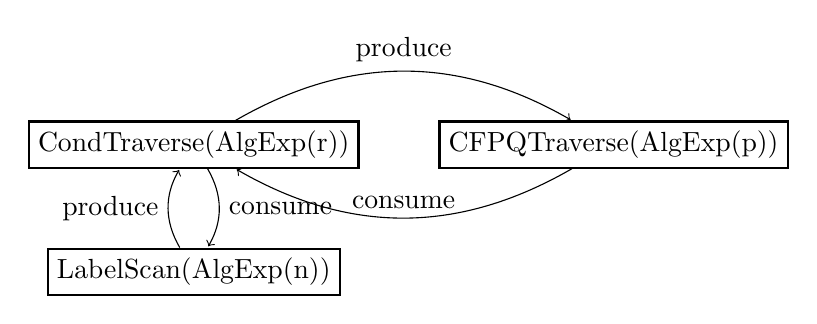
\begin{tikzpicture}[shorten >=0.5pt,auto]
       \node (q_0) [draw,thick,minimum width=2cm,minimum height=0.5cm]                        {LabelScan(AlgExp(n))};
       \node (q_1) [draw,thick,minimum width=2cm,minimum height=0.5cm, above=of q_0]                        {CondTraverse(AlgExp(r))};
        \node (q_2) [draw,thick,minimum width=2cm,minimum height=0.5cm, right=of q_1]                        {CFPQTraverse(AlgExp(p))};
        \path[->]
        (q_0) edge[bend left, left]  node {produce} (q_1)
        (q_1) edge[bend left, right] node {consume} (q_0)
        (q_1) edge[bend left, above] node {produce} (q_2)
        (q_2) edge[bend left, above] node {consume} (q_1);
    \end{tikzpicture}
    \caption{Example of part of the execution plan}
    \label{fig:execution-plan-operations}
\end{figure}


After that we have everything to run multiple-source CFPQ algorithm provided in listing~\autoref{alg:redisgraph-cfpq} to resolve all operation dependencies. This algorithm is slightly different from \textit{MultiSrcCFPQ} algorithm described in listing~\autoref{alg:algo1} and is a generalization of it. It receives the set of operation dependencies \textit{deps} and path pattern context $context$. The algorithm's task is to populate relation and source matrices of all named path pattern from $deps$. To do this on each iteration for all pattern from $deps$ this matrices are updated. Namely, first of all the algebraic expression is constructed from source matrix and algebraic expression of current pattern and then optimized in line~\textbf{5}. This is followed by substitution references in line~\textbf{6}, after which all references in the expression are replaced by relation matrices from $context$. At the end of iteration the resulting expression is evaluated and stored in relation matrix in line~\textbf{7}. These iterations continue as long as the context changes, i.e. at least one of the pattern matrices $m_{rel}$ or $m_{src}$ changes during iteration.

\begin{algorithm}
\begin{algorithmic}[1]
\caption{Multiple-source context-free path querying algorithm in terms of algebraic expressions}
\label{alg:redisgraph-cfpq}
\Function{MultiSrcCFPQAlgExp}{$deps,\ context$}
\While {$context~is~changing$}
    \ForAll{$p~\in deps$}
        \State $src \gets context[p].m_{src}$
        \State $expr \gets$ \Call{Optimize}{$src * context[p].expr$}
        \State \Call{FetchReferences}{$expr$, $ctx$}
        \State $context[p].m_{rel} \gets$ \Call{Eval}{$expr$}
    \EndFor
\EndWhile

\EndFunction
\end{algorithmic}
\end{algorithm}

After running this algorithm on the dependency set of \textit{CFPQTraverse} operation and path pattern context we receive relation matrices of all named path pattern, on which operation depends. For example, after running it on dependency set $\{S\}$, relation and source matrices of pattern $S$ will be as follows:

\begin{align*}
m_{rel} &= \{(3, 5), (3, 6), (4, 5), (4, 6), (5, 5), (5, 6)\} \\
m_{src} &= \{(3, 3), (4, 4), (5, 5)\}
\end{align*}

After that all references in the algebraic expression $p_f *$ \textit{Alg\-Exp(p)} are replaced with the relation matrices and we get algebraic expression $p_f * \mathcal{E}^b * context[S].m_{rel}$. Then this expression is evaluated to matrix $\{(3, 5), (3, 6)\}$ that corresponds to paths from 3rd vertex that satisfy the constraints specified by pattern $S$. Finally as well as \lstinline{CondTraverse}, \lstinline{CFPQTraverse} extracts desired paths from this resulting matrix and passes them to parent operation.

Therefore if we put together the results of all operations of execution plan the query from listing~\ref{lst:cypher-example-3} on graph $D_1$ return the set of vertices $\{(1, 5), (1, 6)\}$.

\subsection{Evaluation}

In order to demonstrate applicability of the provided extension for RedisGraph we evaluate the proposed solution on the subset of cases provided in the section~\ref{sect:py_algo_evaluation}.

For RedisGraph evaluation, we used a PC with Ubuntu 18.04 installed.
It has Intel Core i7-6700 CPU, 3.4GHz, and DDR4 64Gb RAM. 
RedisGraph with our extensions is installed form our GitHub repository\footnote{Sources of RedisGraph database with full-stack CFPQ support:\url{https://github.com/YaccConstructor/RedisGraph/tree/path_patterns_dev}. Access data: 19.07.2020.}. 

\subsubsection{Data preparing}

We use the same graphs which are presented in table~\ref{tbl:graphs_for_cfpq} to evaluate RedisGraph-based solution.

Graphs are loaded into RedisGraph database such that each vertex has a field \verb|id| which value is unique and is in $[0 \ldots |V|-1]$, where $|V|$ is a number of vertices in the graph to load.
This allows us to generate queries for specific chunk size using templates.
The template for the $g_1$ query is provided in listing~\ref{lst:query_pattern_g1}.
Here \texttt{\{id\_from\}} and \texttt{\{id\_to\}} are placeholders for lower and upper bounds for \verb|id|. The example of the exact query for chunk of size 16 is presented in listing~\ref{lst:query_g1}.

\begin{algorithm}
\floatname{algorithm}{Listing}
\begin{algorithmic}[1]
\caption{Cypher query pattern for $g_1$}
\label{lst:query_pattern_g1}
\State PATH PATTERN S =  \par
 \hskip\algorithmicindent ()-/ [<:SubClassOf [$\sim$S | ()] :SubClassOf] \par
 \hskip\algorithmicindent | [<:Type [$\sim$S | ()] :Type] /->()
\State MATCH (src)-/ $\sim$S /->() 
\State WHERE \{id\_from\} <= src.id and src.id <= \{id\_to\}
\State RETURN count(*)
\end{algorithmic}
\end{algorithm}

\begin{algorithm}
\floatname{algorithm}{Listing}
\begin{algorithmic}[1]
\caption{Query $g_1$ in Cypher using the template from listing~\ref{lst:query_pattern_g1}}
\label{lst:query_g1}
\State PATH PATTERN S =  \par
 \hskip\algorithmicindent ()-/ [<:SubClassOf [$\sim$S | ()] :SubClassOf] \par
 \hskip\algorithmicindent | [<:Type [$\sim$S | ()] :Type] /->()
\State MATCH (src)-/ $\sim$S /->() 
\State WHERE 15 <= src.id and src.id <= 31
\State RETURN count(*)
\end{algorithmic}
\end{algorithm}

Queries generator for all three queries ($g_1$, $g_2$, and $geo$) was implemented and used to create queries for all chunks which are used in the previous experiment. 


\subsubsection{Evaluation results}

For evaluation we select $geo$ query for \textit{geospecies} graph as one of the hardest queries, and $g_1$ query for other graphs.
Time and memory consumption are measured for each chunk processing.
Results of time measurement are presented in figures~\ref{fig:redis_core_all}--\ref{fig:redis_gohierarchy_all}.

\begin{figure}[h]
\centering
\includegraphics[width=0.5\textwidth]{data/raw_redis/core.pdf}
\caption{RedisGraph performance of \textit{core} graph}
\label{fig:redis_core_all}
\end{figure}


\begin{figure}[h]
\centering
\includegraphics[width=0.5\textwidth]{data/raw_redis/pathways.pdf}
\caption{RedisGraph performance of \textit{pathways} graph}
\label{fig:redis_pathways_all}
\end{figure}

\begin{figure}[h]core
\centering
\includegraphics[width=0.5\textwidth]{data/raw_redis/enzyme.pdf}
\caption{RedisGraph performance of \textit{enzyme} graph}
\label{fig:redis_enzyme_all}
\end{figure}


\begin{figure}[h]
\centering
\includegraphics[width=0.5\textwidth]{data/raw_redis/go.pdf}
\caption{RedisGraph performance of \textit{go} graph}
\label{fig:redis_go_all}
\end{figure}

\begin{figure}[h]
\centering
\includegraphics[width=0.5\textwidth]{data/raw_redis/geospecies.pdf}
\caption{RedisGraph performance of \textit{geospecies} graph}
\label{fig:redis_geospecies_all}
\end{figure}

\begin{figure}[h]
\centering
\includegraphics[width=0.5\textwidth]{data/raw_redis/eclass_514en.pdf}
\caption{RedisGraph performance of \textit{eclass\_514en} graph}
\label{fig:redis_eclass_all}
\end{figure}

\begin{figure}[h]
\centering
\includegraphics[width=0.5\textwidth]{data/raw_redis/gohierarchy.pdf}
\caption{RedisGraph performance of \textit{gohierarchy} graph}
\label{fig:redis_gohierarchy_all}
\end{figure}

We can see, that results is comparable with one given in section~\ref{sect:py_algo_evaluation}. 
Processing time for all chunks, except chunk of size 10 000 for \textit{geospecies} graph (fig.~\ref{fig:redis_geospecies_all}) is less then 1 second.
Moreover, for chunks of size 16 processing median time is less then 0.1 second, except \textit{geospecies} graph.

Memory consumption is presented in !!!
La-la-la!!!!

Additionally, we measure the time required to process full graph (to solve all-pairs reachability problem) by chunks of size  !!!.
Also, we compare our solution with results of Arseniy Terekhov et al. from~\cite{10.1145/3398682.3399163} which were measured for RedisGraph deployed on the similar hardware and for the same graphs and queries. In~\cite{10.1145/3398682.3399163} Azimov's algorithm was naively integrated with RedisGraph storage without support of query language and other mechanisms such as lazy query evaluation.
Results are provide in the table~\ref{tbl:redis_full_graph_processing}.

\begin{table}
{
\caption{Full graph processing time by RadisGraph with chunks of size !!!, time is measured in seconds (\textbf{Chunks} --- the proposed solution, \textbf{Full} --- results from~\cite{10.1145/3398682.3399163})}
\label{tbl:redis_full_graph_processing}
\small
\rowcolors{2}{black!2}{black!10}
\begin{tabular}{|l|c|c|c|c|c|}
\hline
Graph                       & \#V       & \#E      & Query  & Chunks  &  Full  \\
\hline
\hline
core                        & 1323     & 3636       & $g_1$  & 0.027  &  0.004 \\ 
pathways                    & 6238     & 18 598     & $g_1$  & 0.028  &  0.011 \\ 
gohierarchy                 & 45 007   & 980 218    & $g_1$  & 0.205  &  0.091 \\ 
enzyme                      & 48 815   & 117 851    & $g_1$  & 0.058  &  0.018 \\ 
eclass\_514en               & 239 111  & 523 727    & $g_1$  & 0.198  &  0.067 \\ 
geospecies                  & 450 609  & 2 311 461  & $geo$  & 27.824 &  7.146 \\
go                          & 582 929  & 1 758 432  & $g_1$  & 0.711  &  0.604 \\ 
\hline
\end{tabular}
}
\end{table}

We can see, that chunk-by-chunk processing is 2--7 times slower, but it is still require reasonable time.
For example, it requires more than 200 times less time than solution of Jochem Kuijpers et al.~\cite{Kuijpers:2019:ESC:3335783.3335791} which is based on Neo4j and requires more than 6000 seconds.
Moreover, while solution from~\cite{10.1145/3398682.3399163} requires huge amount of memory (more than 16Gb for \textit{geospecies} graph and $geo$ query), our solution requires only !!! in the same scenario.
Thus it is more suitable for general-purpose graph databases.

Finally we can conclude that provided 
%\section{Evaluation}

This section describes the methodology and answers the following research questions.

\begin{enumerate}
    \item Does fusion via distillation give any benefits at the software and hardware levels?
    \item What are the properties of the generated hardware?
    \item Does the generated hardware outperform software implementations?
\end{enumerate}

\subsection{Methodology}

Our focus is on creating a basis for future research and experiments, thus we make our experiments as much reproducible as possible\footnote{\url{https://github.com/sedwards-lab/fhw/tree/sparse-linear-algebra-distillation/examples/QTreeBenchmarks/diploma/verilog-bool-no-nnz-inlined} (online; accessed:
2022-06-07) Here one could find all the results. For each benchmark all statistics are specified: matrix names, their sizes, collected metrics for both hardware and software benchmarks.}. We benchmarked the following list of chained functions. The choice is prompted by the current state of the distiller: at the moment, it does not successfully distill matrix multiplication. However, the functions are still practical enough, for example, chained addition could be seen in Luby's maximal independent set algorithm and clearly describe the applicability of the proposed approach.

\begin{itemize}
    \item \mintinline{Haskell}{mAdd (==False) (||) (mAdd (==False) (||) m1 m2) m3}
    \item \mintinline{Haskell}{mask (mAdd (== False) (||) m2 m3) (m1)}
    \item \mintinline{Haskell}{map (==Zero) (to_nat) (mAdd (==False) (||) m1 m2}
    \item \mintinline{Haskell}{map (==Zero) (to_nat) (kron (==False) (&&) m1 m2}
\end{itemize}

Above, \mintinline{Haskell}{Zero} and \texttt{to\_nat} are corresponding definitions for Peano arithmetics, since the \texttt{.pot} language does not have any primitives. For the same reason, we operated with boolean matrices. Such functions could be abstracted with free variables and then instantiated in the emitted Haskell code. However, to get maximum from distillation, we provided all the information about the functions. 

For these functions, we compared the execution time of distilled and not distilled hardware generated circuits, execution time of original and distilled Haskell code and reference \textit{Suite Sparse}\footnote{\url{https://github.com/DrTimothyAldenDavis/GraphBLAS} (online; accessed:
2022-06-07), Suite Sparse library sources.}\textsuperscript{,}\footnote{The library also uses different variations of coordinate formats (opaque to the user) and not a quadtree representation.} variants of these functions in C\texttt{++}. Note that SuiteSparse does not support recursive data types, thus only the first two function chains were implemented in SuiteSparse (since Peano number is essentially a linked list). We did not replace Peano numbers with integers, so our experiments could be interpreted easier. For hardware experiments we collected execution time and the number of memory writes and reads, to access how well fusion is performed. For software experiments we only measured the execution time. Also note that we measured only the time, required to execute the lines above, not including any IO, required to get and evaluate function arguments. But in hardware benchmarks we measured the time required to pass arguments into the circuit's memory, because such IO is inevitable. It is tricky to make such measures in Haskell due to laziness, thus the programs were compiled with \texttt{--fno-full-laziness} to turn off memoization. Also all the arguments were forced to normal form via \texttt{force} and \texttt{evaluate}. Haskell programs were compiled\footnote{GHC 8.10.4.} with \texttt{-O2 --fno-full-laziness} and Suite Sparse was compiled with default flags and linked as a shared library to C\texttt{++} code.

We took matrices from SuiteSparse matrix collection with sizes ranging from \texttt{64x64} to \texttt{512x512}. We limited ourselves with such sizes due to the fact that this is the maximum sizes that fit into \texttt{bram} with $2^{16}$ address space. Such number of \texttt{bram} blocks is available only on really expensive FPGA boards, thus in practice sizes would be smaller to achieve better utilization. Once again, it models the situation when data fits into the cache, since \texttt{bram} in our circuits will operate as a cache in real application.

\subsection{Experiments}

Table~\ref{tab:bench_results} shows the results of all execution time benchmarks. To evaluate execution time for hardware simulation, implementation stage was performed to assess the maximum frequency of FPGA device used for synthesis and implementation, and the number of execution cycles was multiplied by the number of nanoseconds a clock cycle takes. The frequencies were equal within the same benchamark set, i.e., frequency was not affected by distillation. We used \texttt{xcu250figd2104-2L} device\footnote{\url{https://www.xilinx.com/products/boards-and-kits/alveo/u250.html}  (online; accessed:
2022-06-07)} for synthesis and implementation stages. It is not really a casual and affordable chip, but it contains enough \texttt{bram} for our evaluation to see scalability. In the table a median across several benchmarks is shown. 

As it could be seen, distillation steadily increases performance: up to 2x speedup for hardware simulation and up to 3x for software benchmarks. The results are maintained within the borders of the corresponding confidence interval and the borders are not shown for brevity. Hardware speedup is lower due to the different execution semantics, dataflow is not reduction-based and distillation is a reduction-based transformation. Note that generated hardware appears to be less performant than both Haskell and C\texttt{++}, which a bit contradicts the results from~\cite{oldfhw}. For hardware benchmarks \texttt{time (IO)} shows the execution time including the time needed to transfer the data though the arguments, \texttt{time (no IO)} does not include it in its turn. It could be seen that not all the benchmarks are computationally extensive enough to cover memory transferring costs, but for more complex examples the ratio would be better. Since we basically transfer the matrices node by node from a file in the testbench, we have probably the lowest possible latency, and in practice it would be higher if reading from DDR, however the bandwidth could be increased. Noticeably, running times for \texttt{mMaskAdd} for C\texttt{++} and distilled Haskell are similar, which shows that fusion really provides some extra performance: SuiteSparse at the moment does not implement any fusion.

Table~\ref{tab:mem_results} summarizes the ratios between distilled and not distilled hardware circuits memory reads and writes. Since in general case distillation removes extra pattern matching, essentially it saves memory reads and writes. The eventual number of memory reads and writes is implementation dependent, thus the table shows what share of speedup is prompted by saving memory operations. Distillation successfully reduces the number of memory accesses, about 15\% on average. \texttt{mMapKron} has a bit higher ratio due to the fact that \texttt{Nat} numbers require additional memory accesses, since the type is recursive. It could also be seen that a major part of speedups is attributed to saved memory accesses. 

Finally, table~\ref{tab:resource_util} shows device resources utilization ratios between distilled and not distilled hardware circuits and frequencies. Columns are device primitives: registers, lookup tables, \texttt{bram} blocks or multiplexers. Utilization for both types of circuits is below 1\% of available resources on the device, except for the memory. Memory blocks utilization is about 30\% (since we choose larger \texttt{brams} to store larger matrices). Apart from that, distilled circuits could have both higher and lower utilization. Since the hardware generation is primarily syntax-directed it follows from the distilled program structure. For example, distillation might glue two recursive functions into one (in that case, memory utilization would be lower, because each cluster of mutually recursive functions possesses its own heap) or make more recursive functions than in the original program. The frequencies are the same, however, they possibly could be made better with more intelligent buffer allocation.

\subsection{Discussion}
Answering the research questions above.

\begin{enumerate}
    \item Fusion gives significant benefits, however at the hardware level the benefits are a bit smaller since hardware semantics is not reduction based. The benefits at the hardware level are mostly determined by the reduced number of memory accesses (each access takes 2 clock cycles). Notably, distilled Haskell implementation of \texttt{mMaskAdd} has similar performance with C\texttt{++}. 
    \item Device utilization is low, but such circuits could be copied on the same device to provide better utilization and higher parallelism. Resource utilization might be both better and worse after distillation, depending on the transformed program itself since translation is syntax-directed. Frequency could be increased by more intelligent buffering strategy.
    \item Although we use low-latency design with \texttt{bram}s that take 2 clock cycles per request and transfer matrices from files, which does not have any latency in simulation, we get slower execution time than Haskell and C\texttt{++} counterparts. It could be partly due to excessive buffering performed by FHW at the moment. Also there is no pipelining for recursive calls, i.e. only one set
of function argument tokens are allowed to enter a tail-recursive function call until a result is finally generated. Further CPS transformation hinders parallelization, which could be made more explicit with SSA. Some other optimizations exist that may significantly influence the performance. Also, since device utilization is about 1\%, such circuits could be copied on one device and provide more parallelism. A more detailed discussion could be found at~\cite{Edwards2019FHWP}.
\end{enumerate}

Distillation clearly showed its applicability to optimization of sparse linear algebra routines and notably it still could be combined with other techniques, like rewrite rules to achieve better results. High-level synthesis has a room for improvements by increasing pipelining, parallelism and frequency and the generated hardware could be improved from usability perspective: a support for arbitrary sized matrices is desirable. Thus we will focus on these directions. Probably a better solution would be to embed \texttt{.pot} language into e.g. Haskell to leverage its type system (to be able to use some rewrite rules as well), and add support for primitive types and parallel primitives to be able to conduct a more scalable comparison with SuiteSparse (since SuiteSparse is multithreaded). For such embedding different execution models could be implemented, including hardware synthesis, for which SSA form of GRIN looks promising, as well as extra optimizations shipped with GRIN. For hardware synthesis, an interesting direction is achieving predictable results in hardware from certain modifications in software. This property partly holds for the current approach, since the translation is syntax- directed. More information on this could be found at~\cite{predict}.

\pagebreak

\begin{table}[t]
\scriptsize
\centering
\caption*{mAddAdd}
\begin{tabular}{|c|c|c|c|c|c|c|c|c|c|} 
\hline
\rowcolor{LightBlue}
\multicolumn{3}{|c|}{Matrices dimensions} & Haskell & Haskell (distilled) & \multicolumn{2}{c|}{FHW} & \multicolumn{2}{c|}{FHW (distilled)} & {C\texttt{++}}\\
% \rowcolor{LightBlue}
\hline
m1 & m2 & m3 & time & time & time (no IO) & time (IO) & time (no IO) & time (IO) & time \\ 
\hline
64 & 64 & 64 & 29 us & 20 us & 76 us & 170 us & 64 us & 158 us & 14 us\\ 
128 & 128 & 128 & 94 & 79 & 146 & 476 & 134 & 469 & 30 \\
256 & 256 & 256 & 123 & 103 & 202 &  681 & 168 & 662 & 44\\
512 & 512 & 512 & 219 & 143 & 474 & 1192 & 375 & 1093 & 49\\
\hline
\end{tabular}

\caption*{mMaskAdd}
\begin{tabular}{|c|c|c|c|c|c|c|c|c|c|} 
\hline
\rowcolor{LightBlue}
\multicolumn{3}{|c|}{Matrices dimensions} & Haskell & Haskell (distilled) & \multicolumn{2}{c|}{FHW} & \multicolumn{2}{c|}{FHW (distilled)} & {C\texttt{++}}\\
% \rowcolor{LightBlue}
\hline
m1 & m2 & m3 & time & time & time (no IO) & time (IO) & time (no IO) & time (IO) & time \\ 
\hline
64 & 64 & 64 & 10 us & 7 us & 64 us & 133 us & 46 us & 111 us & 18 us\\ 
128 & 128 & 128 & 38 & 30 & 118 & 322 & 75 & 292 & 33 \\
256 & 256 & 256 & 48 & 42 & 168 &  498 & 104 & 456 & 46\\
512 & 512 & 512 & 126 & 76 & 400 & 762 & 300 & 729 & 65\\
\hline
\end{tabular}

\caption*{mMapAdd}
\begin{tabular}{|c|c|c|c|c|c|c|c|c|c|} 
\hline
\rowcolor{LightBlue}
\multicolumn{3}{|c|}{Matrices dimensions} & Haskell & Haskell (distilled) & \multicolumn{2}{c|}{FHW} & \multicolumn{2}{c|}{FHW (distilled)} & {C\texttt{++}}\\
% \rowcolor{LightBlue}
\hline
m1 & m2 & m3 & time & time & time (no IO) & time (IO) & time (no IO) & time (IO) & time \\ 
\hline
64 & 64 & --- & 45 us & 37 us & 189 us & 253 us & 137 us & 202 us & ---\\ 
128 & 128 & --- & 162 & 105 & 524 & 685 & 397 & 579 & --- \\
256 & 256 & --- & 312 & 216 & 1047 &  1360 & 680 & 986 & ---\\
512 & 512 & --- & 436 & 273 & 1346 & 1776 & 900 & 1330 & ---\\
\hline
\end{tabular}

\caption*{mMapKron}
\begin{tabular}{|c|c|c|c|c|c|c|c|c|c|} 
\hline
\rowcolor{LightBlue}
\multicolumn{3}{|c|}{Matrices dimensions} & Haskell & Haskell (distilled) & \multicolumn{2}{c|}{FHW} & \multicolumn{2}{c|}{FHW (distilled)} & {C\texttt{++}}\\
% \rowcolor{LightBlue}
\hline
m1 & m2 & m3 & time & time & time (no IO) & time (IO) & time (no IO) & time (IO) & time \\ 
\hline
2 & 64 & --- & 64 us & 36 us & 212 us & 242 us & 94 us & 125 us & ---\\ 
2 & 128 & --- & 137 & 68 & 434 & 502 & 199 & 266 & --- \\
2 & 256 & --- & 364 & 126 & 1004 &  1188 & 449 & 636 & ---\\
4 & 128 & --- & 302 & 94 & 694 & 763 & 330 & 401 & ---\\
\hline
\end{tabular}



\caption{Execution time}
\label{tab:bench_results}

\end{table}
\begin{table}[h]
\scriptsize
\begin{minipage}{0.45\linewidth}
\centering
\caption*{mAddAdd}
\begin{tabular}{|c|c|c|c|c|c|c|} 
\hline
\rowcolor{LightBlue}
\multicolumn{3}{|c|}{Matrices dimensions} & \multicolumn{2}{c|}{Ratio ($\frac{FHW}{FHW_{distilled}}$)}\\
% \rowcolor{LightBlue}
\hline
m1 & m2 & m3 & writes & reads\\ 
\hline
64 & 64 & 64 & 1.10 & 1.15\\ 
128 & 128 & 128 & 1.02 & 1.05\\
256 & 256 & 256 & 1.03 & 1.06\\
512 & 512 & 512 & 1.10 & 1.16\\
\hline
\end{tabular}
\end{minipage}
\begin{minipage}{0.45\linewidth}
\centering
\caption*{mMaskAdd}
\begin{tabular}{|c|c|c|c|c|c|c|} 
\hline
\rowcolor{LightBlue}
\multicolumn{3}{|c|}{Matrices dimensions} & \multicolumn{2}{c|}{Ratio ($\frac{FHW}{FHW_{distilled}}$)}\\
% \rowcolor{LightBlue}
\hline
m1 & m2 & m3 & writes & reads\\ 
\hline
64 & 64 & 64 & 1.13 & 1.26\\ 
128 & 128 & 128 & 1.06 & 1.11\\
256 & 256 & 256 & 1.08 & 1.09\\
512 & 512 & 512 & 1.10 & 1.16\\
\hline
\end{tabular}
\end{minipage}
\begin{minipage}{0.45\linewidth}
\centering
\caption*{mMapAdd}
\begin{tabular}{|c|c|c|c|c|c|c|} 
\hline
\rowcolor{LightBlue}
\multicolumn{3}{|c|}{Matrices dimensions} & \multicolumn{2}{c|}{Ratio ($\frac{FHW}{FHW_{distilled}}$)}\\
% \rowcolor{LightBlue}
\hline
m1 & m2 & m3 & writes & reads\\ 
\hline
64 & 64 & --- & 1.10 & 1.21\\ 
128 & 128 & --- & 1.07 & 1.14\\
256 & 256 & --- & 1.07 & 1.19\\
512 & 512 & --- & 1.10 & 1.21\\
\hline
\end{tabular}
\end{minipage}
\hfill
\begin{minipage}{0.45\linewidth}
\centering
\caption*{mMapKron}
\begin{tabular}{|c|c|c|c|c|c|c|} 
\hline
\rowcolor{LightBlue}
\multicolumn{3}{|c|}{Matrices dimensions} & \multicolumn{2}{c|}{Ratio ($\frac{FHW}{FHW_{distilled}}$)}\\
% \rowcolor{LightBlue}
\hline
m1 & m2 & m3 & writes & reads\\ 
\hline
2 & 64 & --- & 1.71 & 1.88\\ 
2 & 128 & --- & 1.72 & 1.87\\
2 & 256 & --- & 1.65 & 1.83\\
4 & 128 & --- & 1.81 & 1.91\\
\hline
\end{tabular}
\end{minipage}

\caption{Memory accesses}
\label{tab:mem_results}
\end{table}

\begin{table}[h]
\scriptsize
\centering
\begin{tabular}{|l|c|c|c|c|c|c|c|c|c|} 
\hline
\rowcolor{LightBlue}

{Benchmark} & \multicolumn{8}{c|}{Ratio (${\frac{FHW}{FHW_{distilled}}}$)} & {Frequency}\\
\hline
{} & FDRE & LUT3 & LUT6 & LUT5 & LUT4 & LUT2 & RAMB36E2 & MUXF7 & {} \\
% \rowcolor{LightBlue}
\hline
mAddAdd & 0.3 & 0.3 & 0.3 & 0.5 & 0.3 & 0.3 & 0.5 & 0.5 & 200 MHz\\ 
mMaskAdd & 0.5 & 0.5 & 0.7 & 0.4 & 0.7 & 0.5 & 0.7 & 0.6 & 200 MHz\\
mMapAdd & 1 & 0.9 & 0.9 & 1.2 & 1 & 1.1 & 1.1 & 1.2 & 200 MHz\\
mMapKron & 1.5 & 1.5 & 1.3 & 2 & 2 & 1.8 & 1.4 & 1.7 & 200 MHz\\
\hline
\end{tabular}
\caption{Resource utilization}
\label{tab:resource_util}
\end{table}
\pagebreak

\section{Conclusion and Future Work}

We present !!!

Our evaluation shows that !!!

First direction for future research is a more detailed CFPQ algorithms investigation.
We should do More evaluation on sparse matrices on GPGPUs.

Also it is nesessary to implement and evaluate solutions for graphs which is not fit in RAM.
There is a set of technics for huge matrices multiplication.
Is it possible to dopt it for CFPQ

Another direcion is a dataset improvement.
More data.
More grammars/queries.


\section*{Acknowledgements}
Grants

Thanks to Ekaterina Verbitskaia for paper improvements and fruitful discussion.

Thanks to Roi Lipman for his help with RedisGraph internals investigation and for his comment on impractical memory consumption of the original Aziomv's algorithm which motivates us to develop the described solution.

Anonimus reviewers !!!

%%
%% The next two lines define the bibliography style to be used, and
%% the bibliography file.
\bibliographystyle{ACM-Reference-Format}
\bibliography{main}

%%
%% If your work has an appendix, this is the place to put it.
%% Please note that all the content must fit within the page limits, including any appendices.
%\appendix
%
%\section{Research Methods}
% ...

\end{document}
\endinput


